\chapter{Asking Millionaires How To Make \$1{,}000{,}000!}

This chapter follows a School of Hard Knocks interview, curated by LazyingArt LLC. The source is not a blackboard lecture but a moving search through wealthy Austin neighborhoods, so we proceed a little differently than usual. We keep the order of the encounters, the refusals, the resets, and the strongest answers, and we extract from them a compact mathematical spine: persistence under low hit rates, the accumulation of savings, the choice between labor and ownership, the fit between business format and market, and the way optionality widens when financial runway grows.

\begin{remark}
No validated lecture screenshots survive for this chapter. The equations and diagrams below are therefore editorial reconstructions of the spoken logic, not transcriptions of visible board work.
\end{remark}

\section{Opening the Inquiry}

The lecture begins as a field experiment. We are told, in plain language, that the goal is to go around one of the wealthiest neighborhoods in Texas and ask millionaires how they became wealthy. That opening matters because it establishes both the ambition and the method: we are not reading a polished retrospective but watching the host try to extract usable rules from people who may or may not wish to talk.

The first house does not yield an interview. That is not a disposable scene. It tells us that the cost of the inquiry is immediate. Before we learn any business principle, we learn that the search for principles itself runs through refusal, awkwardness, and repetition. Later the host says the success rate is easily below five percent, which we may preserve as
\begin{equation}
p_{\text{successful interview}} < 0.05.
\end{equation}
The inequality is simple, but its role in the lecture is structural. The host is already teaching one of the rules the interviewees will later repeat: one does not get to the useful answer without passing through a great many unusable ones.

\begin{figure}[h]
\centering
\begin{tikzpicture}[x=2.7cm,y=1cm]
\node[draw, rectangle, minimum width=2.3cm, minimum height=0.8cm] (ask) at (0,0) {Knock / Ask};
\node[draw, rectangle, minimum width=2.3cm, minimum height=0.8cm] (rej) at (2.3,0) {Rejection};
\node[draw, rectangle, minimum width=2.3cm, minimum height=0.8cm] (reset) at (4.6,0) {Reset / Reframe};
\node[draw, rectangle, minimum width=2.3cm, minimum height=0.8cm] (next) at (6.9,0) {Next Door};

\draw[->] (ask) -- (rej);
\draw[->] (rej) -- (reset);
\draw[->] (reset) -- (next);
\draw[->, bend left=35] (next.north) to node[above] {repeat} (ask.north);
\end{tikzpicture}
\caption{Editorial schematic of the lecture's opening method: the search itself is iterative, and the episode treats that iteration as part of the lesson.}
\end{figure}

This gives the chapter its first rhythm. We ask. We are refused. We say, in effect, no worries. Then we continue. The inquiry is already procedural before it becomes conceptual.

\section{Apprenticeship, Difficulty, and the First Money}

The first substantial answer comes from a man who pursued natural gas. His advice is severe: choose the most difficult, most challenging, most dangerous job you can find; work harder than anybody else; and if you see a problem, do not wait for someone else to fix it. That answer appears early because the lecture wants a blunt first rule after a refusal. It gives us an ethic of entry.

\paragraph{Anecdote.}
The speaker chose natural gas and describes it in the language of risk and difficulty.

\paragraph{Claim.}
The rule is not merely ``work hard.'' The stronger claim is that wealth begins by moving toward difficult domains and taking ownership of problems inside them.

\paragraph{Mechanism.}
The mechanism can be written schematically as
\begin{align}
\text{difficulty} &\longrightarrow \text{initiative} \longrightarrow \text{responsibility}, \\
\text{problem noticed} &\longrightarrow \text{cause identified} \longrightarrow \text{value created}.
\end{align}
When the host asks for the most money made in a single year, the answer is given as cash flow of about half a million dollars:
\begin{equation}
C_{\text{cash flow}} \approx \$5\times 10^{5}\ \text{yr}^{-1}.
\end{equation}
The number matters not because it is spectacular, but because it ties the ethic of difficult work to a concrete operating outcome.

The next interview complicates the first one in a useful way. A software executive says that his first job out of college was at a startup and that this was a great education, but if he had to do it again he might first work at a large company, learn best practices there, and only then return to a smaller firm. The lecture is now setting up a real apprenticeship problem. Is the right first move raw struggle in a demanding industry, or structured learning inside an institution that already knows how to operate?

We can summarize that second path as
\begin{equation}
\text{large firm} \longrightarrow \text{best practices} \longrightarrow \text{smaller-firm leverage}.
\end{equation}
The same interview adds another practical rule: begin in a city with many options so that one can move from company to company rather than becoming trapped in a thin market. We should preserve that point because it is not a decorative aside. It is an argument that career mobility itself is a form of optionality.

\section{Ownership Versus Employment}

After another refusal, the host narrates the low hit rate and then returns for day two. This reset should remain visible in the notes. It is the moment when the lecture turns the social difficulty of the project into motivation. We are still getting no's, but the host insists that the search is worth continuing. Only after this reset does the lecture arrive at its strongest answer.

A former professional basketball player, now part of a sports ownership group with teams around the world, is asked for his best entrepreneurial advice. The answer is immediate and forceful: do not work for anyone if you can avoid it; find something you are passionate about; and if you are going to spend your time on something, spend it growing something that is truly yours. The lecture is no longer speaking merely about income. It is speaking about the structure of the claim one has on the thing one is building.

\begin{definition}
We shall call \emph{optionality} the size of the set of serious career and business moves one can take without immediate financial distress.
\end{definition}

The interview then adds the indispensable qualifier. Ownership is hard when one is young. One may first have to work, save aggressively, and only then commit the time to building something owned. The argument is therefore sequential, not impulsive.

\begin{figure}[h]
\centering
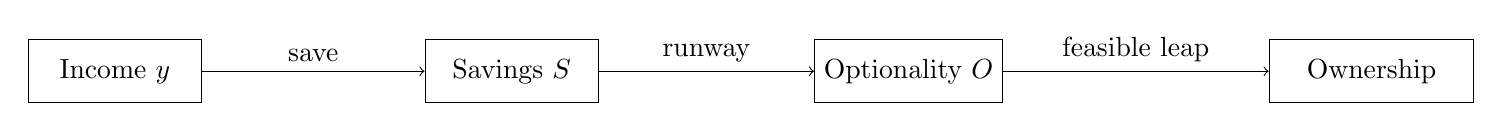
\begin{tikzpicture}[x=2.8cm,y=1.1cm]
\node[draw, rectangle, minimum width=2.2cm, minimum height=0.8cm] (income) at (0,0) {Income \(y\)};
\node[draw, rectangle, minimum width=2.2cm, minimum height=0.8cm] (savings) at (1.8,0) {Savings \(S\)};
\node[draw, rectangle, minimum width=2.2cm, minimum height=0.8cm] (option) at (3.6,0) {Optionality \(O\)};
\node[draw, rectangle, minimum width=2.6cm, minimum height=0.8cm] (own) at (5.7,0) {Ownership};

\draw[->] (income) -- node[above] {save} (savings);
\draw[->] (savings) -- node[above] {runway} (option);
\draw[->] (option) -- node[above] {feasible leap} (own);
\end{tikzpicture}
\caption{Editorial summary of the lecture's main chain: labor income finances savings; savings widen optionality; optionality makes ownership attempts feasible.}
\end{figure}

The host briefly calls this his favorite interview so far. That cue should not be ignored. The episode itself is marking this as a local peak.

\subsection{Question \& Answer}

\paragraph{Question.}
If ownership is the superior long-run position, why does the lecture not simply tell us to leave salaried work at once?

\paragraph{Answer.}
Because the obstacle is not desire but feasibility. The interviewer's question opens the issue at the level of ambition, but the answer closes it at the level of runway. One works, saves, and then uses the saved surplus to create the time and freedom required for ownership.

Let \(S(t)\) be savings at time \(t\), \(y\) labor income flow, \(s\) the savings rate, and \(c\) the consumption outflow. In continuous-time shorthand, the spoken mechanism may be written as
\begin{equation}
S(t+\Delta t)=S(t)+s\,y\,\Delta t-c\,\Delta t.
\end{equation}
What matters is not the notation itself but the monotonic relation it makes visible:
\begin{equation}
O=O(S), \qquad \frac{dO}{dS}>0.
\end{equation}
More savings mean more runway, and more runway means more choices. That is precisely the intuition the lecture returns to at the end.

To make the mechanism explicit, let us pass to yearly units and define the annual surplus
\begin{equation}
\sigma = s\,y-c.
\end{equation}
Then the discrete update becomes
\begin{align}
S_{n+1} &= S_n + \sigma, \\
S_n &= S_0 + n\sigma.
\end{align}
If one needs a threshold \(S^\star\) before leaving pure employment to build something owned, the first feasible year \(n\) satisfies
\begin{equation}
n \ge \frac{S^\star-S_0}{\sigma}.
\end{equation}
This is the lecture's answer in a more compact language. Ownership is not opposed to patience; ownership is often financed by patience.

It is then natural to summarize the broader path by the accounting identity
\begin{equation}
W \approx W_{\text{labor}} + W_{\text{ownership}},
\end{equation}
where the lecture clearly prefers the second term over the long run, not because wages are useless, but because wages may finance the transition into scalable claims.

\section{Scale, Planning, and the Reading of Character}

The next interview widens the scene from personal ownership to large-scale business construction. We hear of a broadcasting group of roughly 350 radio stations, of a first station bought at age twenty-nine, and of a year in which the sale of the business produced something like fifty million dollars:
\begin{equation}
X_{\text{company sale}} \approx \$5\times 10^{7}.
\end{equation}
Again the lecture handles the spectacle carefully. It gives us the large number, but it does not let the number itself become the lesson.

\paragraph{Anecdote.}
A very large exit is reported, and the scale of the enterprise is emphasized.

\paragraph{Claim.}
The durable mechanism is not simply ``have a big year.'' It is to communicate well, connect to the right people, build a strong team, trust them, and have a good business plan.

\paragraph{Mechanism.}
The interview then becomes more discriminating. When asked what one should look for in employees or business partners, the answer is striking: look for somebody who has had some failure. The rationale is that one learns more about character from the fall and the recovery than from uninterrupted smoothness. In compressed form,
\begin{equation}
\text{failure} + \text{recovery} \Longrightarrow \text{evidence about character}.
\end{equation}
This is not a formal theorem, but it is a real selection rule. The episode is moving from success stories to the criteria by which people and plans should be judged.

\section{Market Homework and Local Fit}

At this point the lecture pivots again. The host remarks on how strange the whole project must look from the homeowners' point of view: people are going door to door in very expensive neighborhoods asking for interviews. This aside is important because it performs a second reset. Then the next interview drives us away from inspirational abstraction and toward market realism.

A trial lawyer, who says he also once owned part of three bars in Houston, offers the strongest applied business example in the episode. His advice is succinct: do your homework. The illustration is a new pizza place in Westlake. At first this sounds unremarkable. The revealing detail is that it sells slices. The objection is then sharpened: slices work in a place like Times Square, where passing foot traffic is dense; they are far less natural in a quieter pocket near a supermarket in Westlake.

This gives us the chapter's clearest market-fit statement. Let \(D\) be local demographics, \(F\) local foot traffic, and \(P\) product format. Then the spoken logic is
\begin{equation}
D_{\text{local demographics}} \text{ and } F_{\text{foot traffic}} \text{ must fit } P_{\text{product format}}.
\end{equation}
We may summarize the same thought more compactly by
\begin{equation}
M = M(D,F,P),
\end{equation}
where \(M\) is market fit.

\begin{figure}[h]
\centering
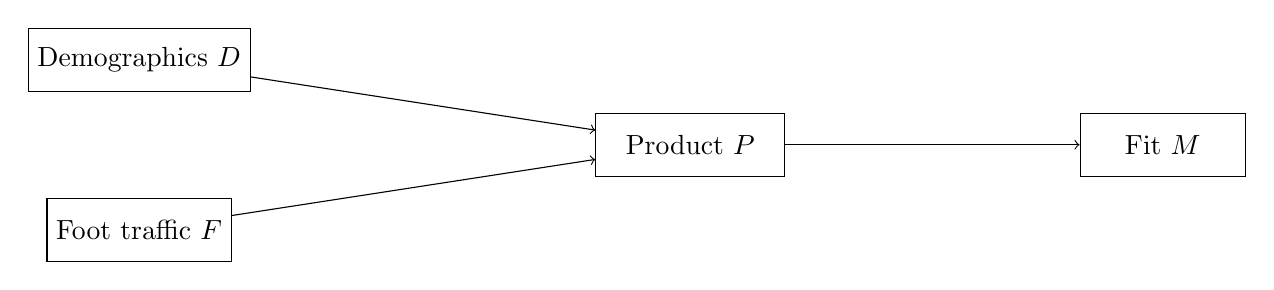
\begin{tikzpicture}[x=2.5cm,y=1.2cm]
\node[draw, rectangle, minimum width=2.2cm, minimum height=0.8cm] (d) at (0,0.9) {Demographics \(D\)};
\node[draw, rectangle, minimum width=2.2cm, minimum height=0.8cm] (f) at (0,-0.9) {Foot traffic \(F\)};
\node[draw, rectangle, minimum width=2.4cm, minimum height=0.8cm] (p) at (2.8,0) {Product \(P\)};
\node[draw, rectangle, minimum width=2.1cm, minimum height=0.8cm] (m) at (5.2,0) {Fit \(M\)};

\draw[->] (d) -- (p);
\draw[->] (f) -- (p);
\draw[->] (p) -- (m);
\end{tikzpicture}
\caption{Editorial reconstruction of the lecture's local-fit diagnostic: a business model is judged not in the abstract but against the neighborhood that must sustain it.}
\end{figure}

The episode's reasoning may then be written as a short decision chain:
\begin{enumerate}
\item Specify the business format \(P\).
\item Ask what sort of customer flow \(F\) that format requires.
\item Ask whether the local population \(D\) and its habits will support that flow.
\item If not, the enterprise may already be weak before management quality is considered.
\end{enumerate}
The force of the example is that nothing mystical is needed. A business may fail because it was never well matched to the neighborhood that had to carry it.

\section{Skill, Capital, and the Long Horizon}

The next sequence broadens the evidence while keeping the lecture's rhythm of short, transferable rules. One interviewee says he founded two technical companies, one acquired by Intel and one, MyVest, acquired by TIAA. His advice is stripped down to a nearly austere form: learn a great deal, acquire a marketable skill, and master it. The lecture is insisting here that before capital scales, competence must exist.

From there the episode turns to investing. The interviewee says timing is difficult. That point is crucial. Rather than pretending that one can reliably call the market, he replaces a timing rule with a horizon rule: capital should be money one will not need for perhaps ten years. In compact form,
\begin{equation}
T_{\text{investment horizon}} \approx 10\ \text{years}.
\end{equation}
The logic is not that ten years is magical. The logic is that the commitment must be made with capital that does not need near-term liquidity. The lecture is changing the question from ``Can we predict well?'' to ``Can we wait long enough?''

When asked about the most money made in a single year, the answer is intentionally vague: seven digits, but no more. The cleanest faithful notation is therefore interval-valued:
\begin{equation}
Y_{\max} \in [10^{6},10^{7}) \text{ dollars}.
\end{equation}

A professor with a software-engineering background later says that long-term real-estate investing was a good financial decision. The humorous comment about marrying a successful lawyer should remain in the chapter as color, but not as a principle. The principle is the same one we have already seen from a different angle: long-term position matters more than near-term flair.

\section{Persistence, Conviction, Reputation, and Optionality}

The final third of the lecture comes as a fast sequence of smaller interviews, but it is not random. It is cumulative. We first hear from someone in sales: what separates people is persistence, the willingness to keep going, and, crucially, the willingness to reevaluate when something is not working. The lecture is careful here. Persistence is not blind repetition. It is repeated effort with adaptation.

That point echoes the episode's opening method. The host kept knocking. The sales professional says to do the same in commercial life, but to remain corrigible. In that sense, the lecture's own structure becomes one of its arguments.

The next interview, with a real-estate developer in Austin, drives the lesson into a sharper operational form. Know what you are going after. Know your market. Make fast decisions. Have conviction. Yet that same answer is immediately bounded by another principle: keep a good name, keep a good reputation, and treat investors properly.

If \(R_t\) denotes reputation capital at time \(t\), we may summarize the lecture's constraint as
\begin{equation}
R_{t+1}=R_t+\Delta R_{\text{good conduct}}-\Delta R_{\text{bad conduct}}.
\end{equation}
The formula is schematic, but its meaning is clear. Speed is not a substitute for trust. Conviction that burns reputation is not mastery; it is decay.

The same interview then widens the map of real estate itself. There is opportunity in many layers of the field: cutting lawns, buying and selling properties, buying land, and development. The lecture is careful not to fetishize one glamorous slot. The deeper rule is to understand the part of the market one is entering and then to move through it with speed, judgment, and consistency.

Finally the host asks how someone can start becoming wealthy now. The answer circles back to the savings argument in a more personal form. When the speaker began his brokerage career with a partner, he had enough savings to make the commitment. Without that accumulated buffer, the choice would not have existed. This is where the lecture's recurring theme becomes fully explicit: without financial stability, one loses optionality.

We may therefore restate the final mechanism, now with the full chapter behind it:
\begin{equation}
\frac{dO}{dS}>0.
\end{equation}
Savings are not glamorous in the episode. They are structural. They enlarge the feasible set of lives one can actually choose.

\section{Summary}

The lecture begins with doors, refusals, and a very low success rate, and that opening is already part of the teaching. We first learn that useful rules are extracted under rejection. We then hear two early answers about apprenticeship: one pushes toward difficult work and problem ownership, the other toward best practices and institutional learning. After a day-two reset, the lecture reaches its strongest answer: one should not merely spend a career building for someone else if it is possible, with patience and savings, to build something one can own.

From there the chapter descends from aspiration into mechanism. Large outcomes depend on people, plans, communication, and trust. Character may be read in recovery after failure. Markets must fit their neighborhoods. Skill must precede leverage. Investing requires horizon more than bravado. Persistence must be paired with reevaluation. Conviction must be paired with reputation. And the closing point gathers all the others: savings are valuable because they preserve optionality.

The lecture therefore does not present a secret formula for instant wealth. It presents a sequence of constraints and practices by which the set of available futures becomes wider rather than narrower.